% ============================================================
% MMM 5162 - Modelling and Simulation
% Mini Project 1 - MR Track
% Compile with XeLaTeX
% ============================================================

\documentclass[12pt,a4paper]{article}

% ---------- Page and text formatting ----------
\usepackage[a4paper,margin=2.5cm]{geometry}
\usepackage{fontspec}
\usepackage{polyglossia}
\setdefaultlanguage{english}
\setotherlanguage{arabic}

\IfFontExistsTF{Times New Roman}
  {\setmainfont{Times New Roman}}
  {\setmainfont{TeX Gyre Termes}}

\newfontfamily\arabicfont[Script=Arabic]{Amiri}

\usepackage{setspace}
\onehalfspacing

\usepackage{ragged2e}
\AtBeginDocument{\justifying}

\usepackage{titlesec}
\titleformat{\section}
  {\bfseries\fontsize{14}{16}\selectfont}
  {\thesection.}{0.5em}{}
\titleformat{\subsection}
  {\bfseries\itshape\fontsize{12}{14}\selectfont}
  {\thesubsection}{0.5em}{}

\usepackage{graphicx}
\usepackage{booktabs}
\usepackage{array}
\usepackage{amsmath}
\usepackage{siunitx}
\usepackage{caption}
\usepackage{float}
\usepackage{fancyhdr}
\usepackage{enumitem}
\usepackage{xcolor}

% ---------- Captions ----------
\captionsetup{
  font=small,
  labelfont=bf,
  justification=centering
}

% ---------- Footer ----------
\pagestyle{fancy}
\fancyhf{}
\cfoot{\thepage}
\renewcommand{\headrulewidth}{0pt}
\renewcommand{\footrulewidth}{0pt}

% ---------- Spacing ----------
\setlength{\parindent}{1.25em}
\setlength{\parskip}{0pt}
\setlength{\textfloatsep}{8pt}
\setlength{\floatsep}{8pt}
\setlength{\intextsep}{8pt}

% ---------- User details: EDIT THESE ----------
\newcommand{\studentname}{Mohammed Rasheed}
\newcommand{\studentid}{481011696}
\newcommand{\submissiondate}{12 Sep}

\begin{document}

% ============================================================
% TITLE PAGE
% ============================================================
\begin{titlepage}
\thispagestyle{empty}
\centering

\renewcommand{\arraystretch}{1.35}
\begin{tabular}{|>{\centering\arraybackslash}m{0.37\textwidth}|
                >{\centering\arraybackslash}m{0.18\textwidth}|
                >{\centering\arraybackslash}m{0.37\textwidth}|}
\hline
\textbf{\large Islamic University of Madinah}\\
\textbf{\large Faculty of Engineering}\\
\textbf{\large Department of Electrical Engineering}
&
\IfFileExists{ium_logo.png}
  {
\includegraphics[height=2.7cm]{ium_logo.png}}
  {\textbf{IUM}}
&
\textarabic{\Large الجامعة الإسلامية}\\
\textarabic{\Large كلية الهندسة}\\
\textarabic{\Large قسم الهندسة الكهربائية}
\\
\hline
\end{tabular}

\vspace{0.8cm}

{\bfseries\Large MMM 5162 -- Modelling and Simulation\par}
\vspace{0.35cm}
{\bfseries\large Mini Project 1\par}
\vspace{0.2cm}
{\bfseries\large Computational Simulation and Parameter Study\par}
\vspace{0.25cm}
{\bfseries [CLO 3.1, PLO V2]\par}

\vspace{1.0cm}

{\bfseries\LARGE Two-Link Robot Pick-Cycle Kinematic Simulation\par}
\vspace{0.3cm}
{\bfseries\large Track MR, Student-Specific Case \(S=18\)\par}

\vfill

{\bfseries\large Submitted To\par}
\vspace{0.1cm}
{\bfseries\large Prof. Adel Abdennour\par}

\vfill

{\bfseries\large Student's Name\par}
\vspace{0.1cm}
{\large \studentname\par}
{\large Student ID: \studentid\par}

\vfill

{\bfseries\large Date\par}
\vspace{0.1cm}
{\large \submissiondate\par}

\vspace{0.6cm}
\hrule
\vspace{0.15cm}
{\small\itshape MMM 5162 -- Modelling and Simulation}

\end{titlepage}

% Page 1 begins here, as required by the report-format rules.
\setcounter{page}{1}

% ============================================================
% 1. INTRODUCTION
% ============================================================
\section{Introduction}

This mini-project implements and evaluates the kinematic motion of a two-link planar robot during one smooth pick-and-place cycle. The objective is to represent the supplied cubic joint-motion model as a reusable Python function, simulate the assigned baseline case for \(S=18\), and perform a controlled study of cycle time. The study compares the nominal cycle with faster and slower motions in order to quantify the effect of cycle duration on joint-speed requirements while verifying that the prescribed geometric trajectory remains unchanged.

% ============================================================
% 2. THEORY / MODELLING
% ============================================================
\section{Theory/Modelling}

For \(S=18\), the assigned parameters are \(L_1=0.470~\mathrm{m}\), \(L_2=0.372~\mathrm{m}\), \(q_{1,start}=38^\circ\), \(q_{1,end}=66^\circ\), \(q_{2,start}=-40.6^\circ\), \(q_{2,end}=24^\circ\), and nominal cycle time \(T=3.12~\mathrm{s}\). Angles are converted to radians before calculation. The normalized time and cubic motion law are
\[
u=\frac{t}{T}, \qquad s(u)=3u^2-2u^3,
\]
and each joint angle is calculated from
\[
q_j(t)=q_{j,start}+\left(q_{j,end}-q_{j,start}\right)s(u), \qquad j=1,2.
\]
Differentiating the motion law gives
\[
\dot q_j(t)=\left(q_{j,end}-q_{j,start}\right)
\frac{6u-6u^2}{T}.
\]
The end-effector coordinates are obtained using the supplied forward-kinematic model
\[
x=L_1\cos q_1+L_2\cos(q_1+q_2), \qquad
y=L_1\sin q_1+L_2\sin(q_1+q_2).
\]

% ============================================================
% 3. SIMULATION AND DESIGN METHODS
% ============================================================
\section{Simulation and Design Methods}

Python 3.13 was used with NumPy for numerical arrays, pandas for tabulated results, and Matplotlib for figures. The engineering equations were implemented in a separate function file, \texttt{robot\_model.py}, while \texttt{main\_simulation.py} generated 1001 equally spaced time samples, executed the experiments, calculated performance measures, saved the results, and performed verification checks. Three cycle durations were studied: \(0.8T=2.496~\mathrm{s}\), \(T=3.120~\mathrm{s}\), and \(1.2T=3.744~\mathrm{s}\).

The program automatically rejects non-positive link lengths, non-positive cycle times, and time values outside the interval \(0\leq t\leq T\). It also verifies the initial and final joint angles and confirms zero joint velocity at the start and end of every cycle. Figures~\ref{fig:path} and~\ref{fig:velocity} show the principal baseline responses.

\begin{figure}[H]
\centering
\begin{minipage}[t]{0.48\textwidth}
\centering
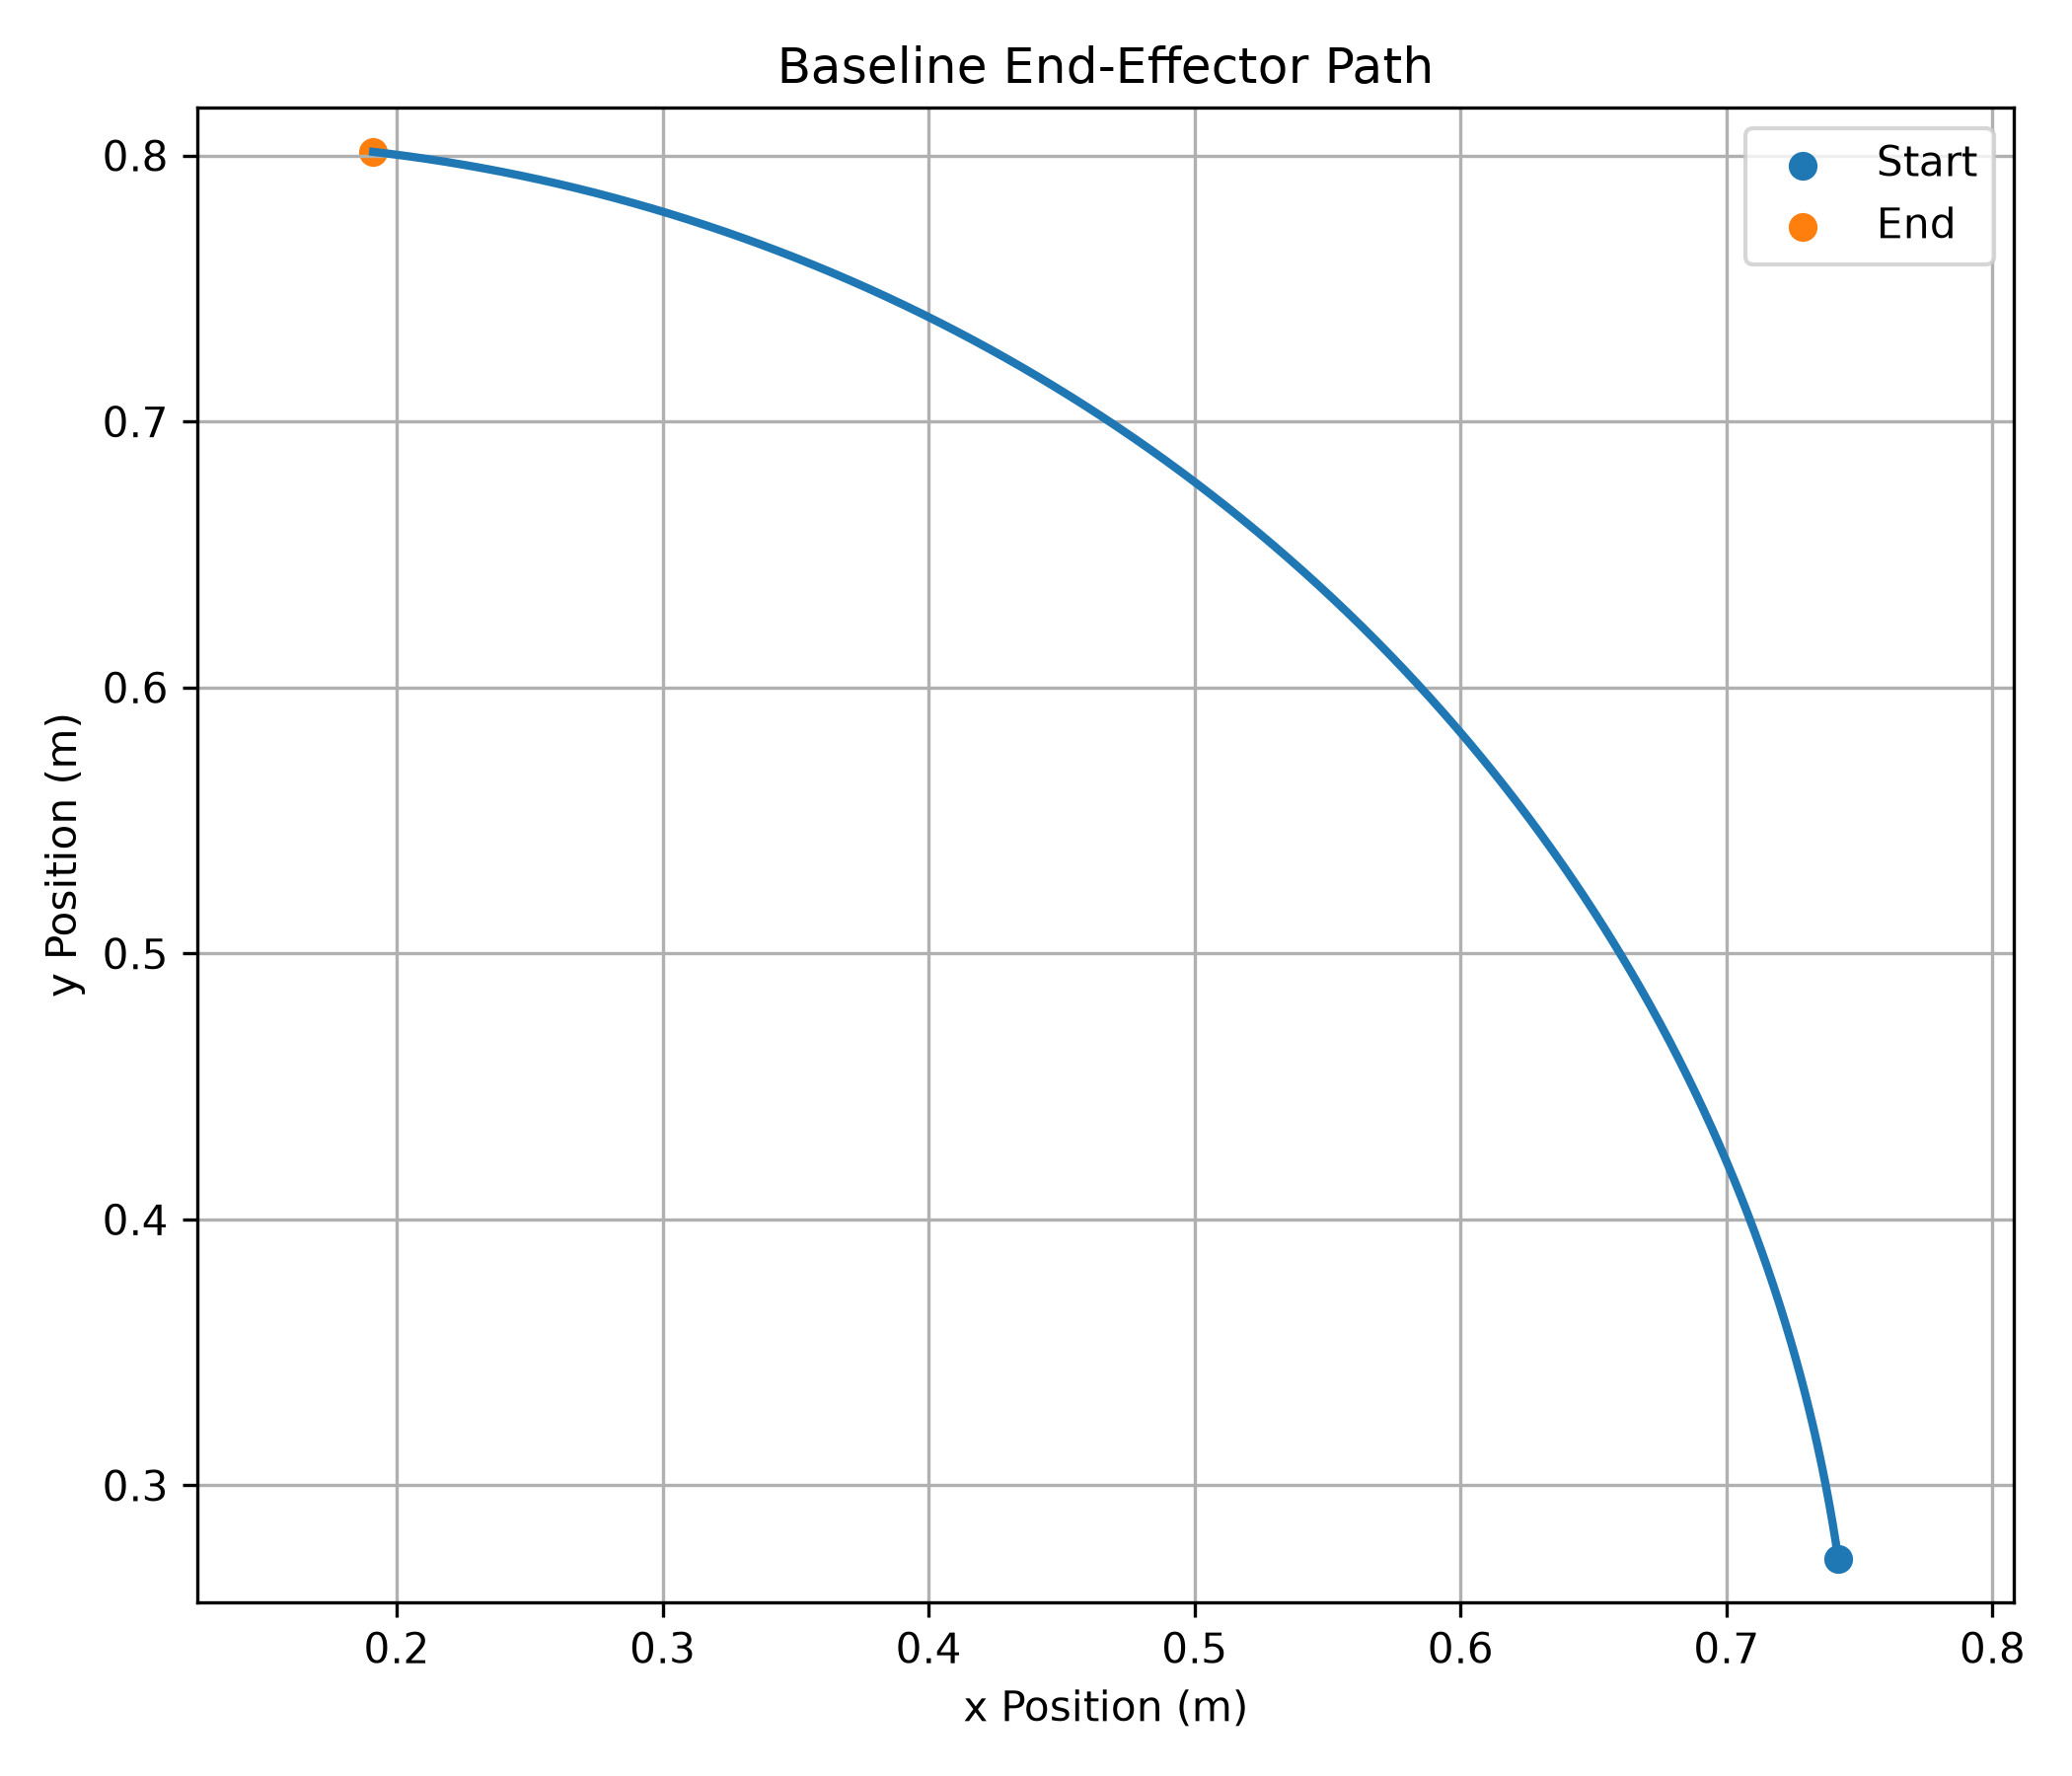
\includegraphics[width=\linewidth]{../results/figures/baseline_end_effector_path.png}
\caption{Baseline end-effector path for \(T=3.12~\mathrm{s}\).}
\label{fig:path}
\end{minipage}
\hfill
\begin{minipage}[t]{0.48\textwidth}
\centering
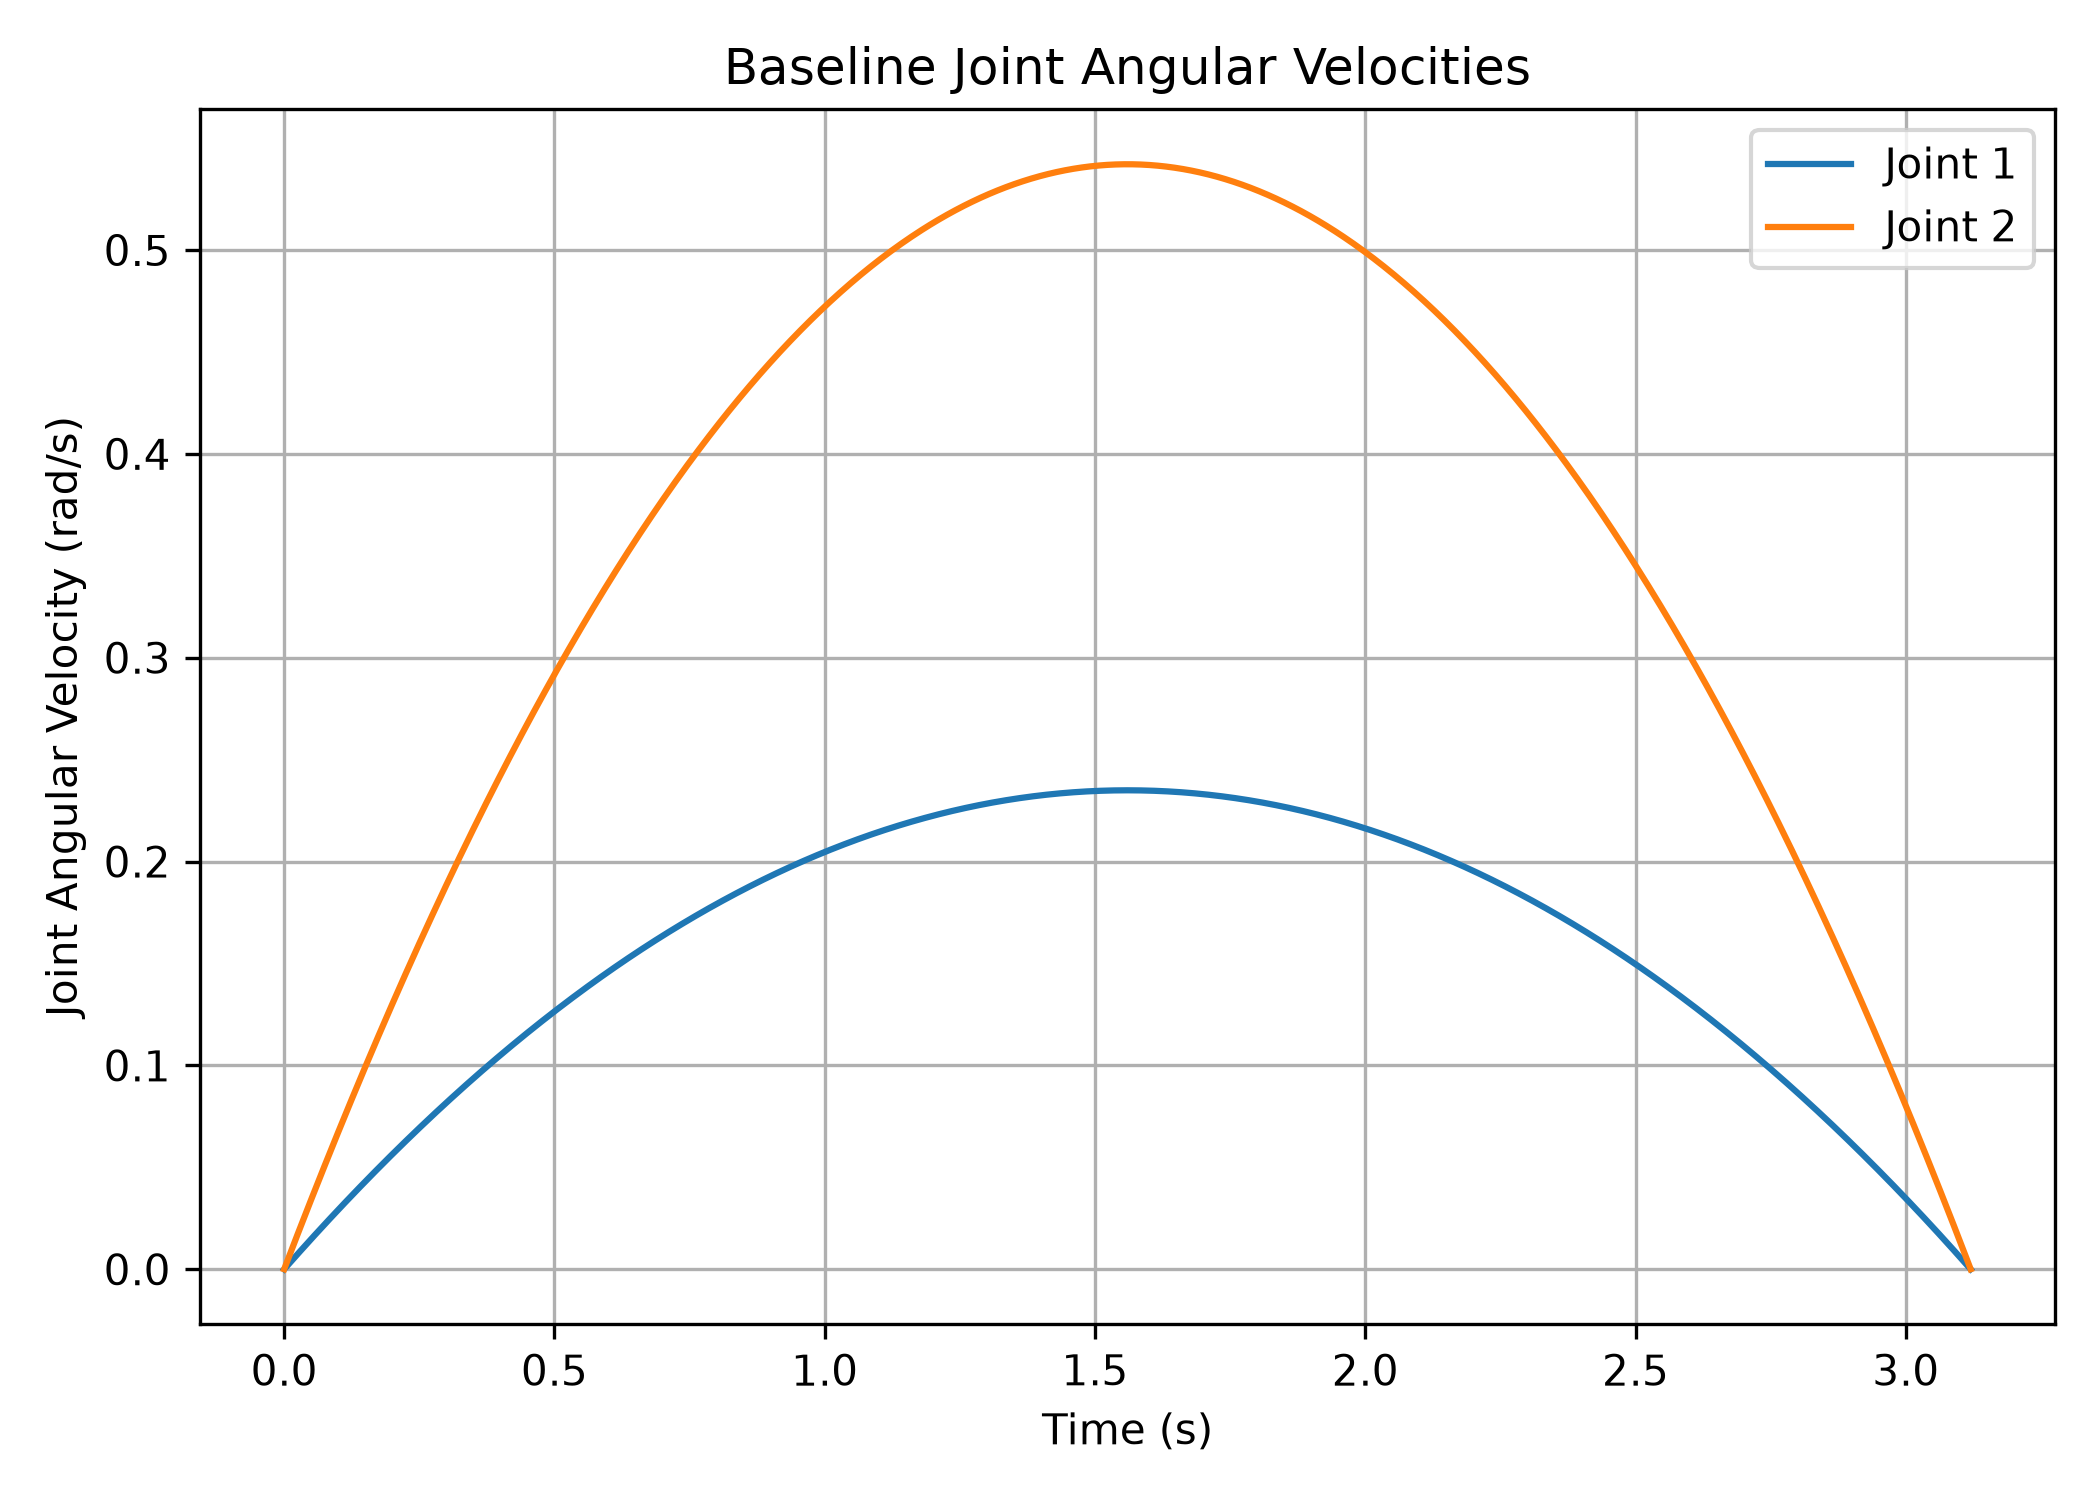
\includegraphics[width=\linewidth]{../results/figures/baseline_joint_velocities.png}
\caption{Baseline joint angular velocities.}
\label{fig:velocity}
\end{minipage}
\end{figure}

% ============================================================
% 4. DISCUSSION / CONCLUSIONS
% ============================================================
\section{Discussion/Conclusions}

Table~\ref{tab:results} summarizes the quantitative results. The baseline maximum joint speeds are \(0.23495~\mathrm{rad/s}\) for Joint~1 and \(0.54206~\mathrm{rad/s}\) for Joint~2. Reducing the cycle time to \(0.8T\) raises both maximum joint speeds by 25\%, whereas increasing the cycle time to \(1.2T\) reduces them by approximately 16.7\%. The maximum end-effector speed follows the same trend, changing from \(0.39869~\mathrm{m/s}\) at the nominal cycle to \(0.49836~\mathrm{m/s}\) for \(0.8T\) and \(0.33224~\mathrm{m/s}\) for \(1.2T\).

\begin{table}[H]
\centering
\caption{Parameter-study performance measures.}
\label{tab:results}
\small
\begin{tabular}{lrrrr}
\toprule
Case & \(T\) (s) & Max. \(|\dot q_1|\) & Max. \(|\dot q_2|\) & Path (m)\\
 & & (rad/s) & (rad/s) & \\
\midrule
\(0.8T\) & 2.496 & 0.29369 & 0.67757 & 0.82045\\
\(T\)    & 3.120 & 0.23495 & 0.54206 & 0.82045\\
\(1.2T\) & 3.744 & 0.19579 & 0.45172 & 0.82045\\
\bottomrule
\end{tabular}
\end{table}

The end-effector path length remains \(0.82045~\mathrm{m}\) in all three cases, and the end-effector coordinates remain approximately \((0.74198,0.27249)~\mathrm{m}\) at the start and \((0.19117,0.80137)~\mathrm{m}\) at the end. This occurs because the motion is parameterized by normalized time \(u=t/T\); changing \(T\) changes how quickly the same sequence of joint configurations is traversed but does not change the configurations themselves. Figure~\ref{fig:comparison} therefore provides the main engineering conclusion: shorter robot cycles demand higher actuator speed even when the geometric task is unchanged.

\begin{figure}[H]
\centering
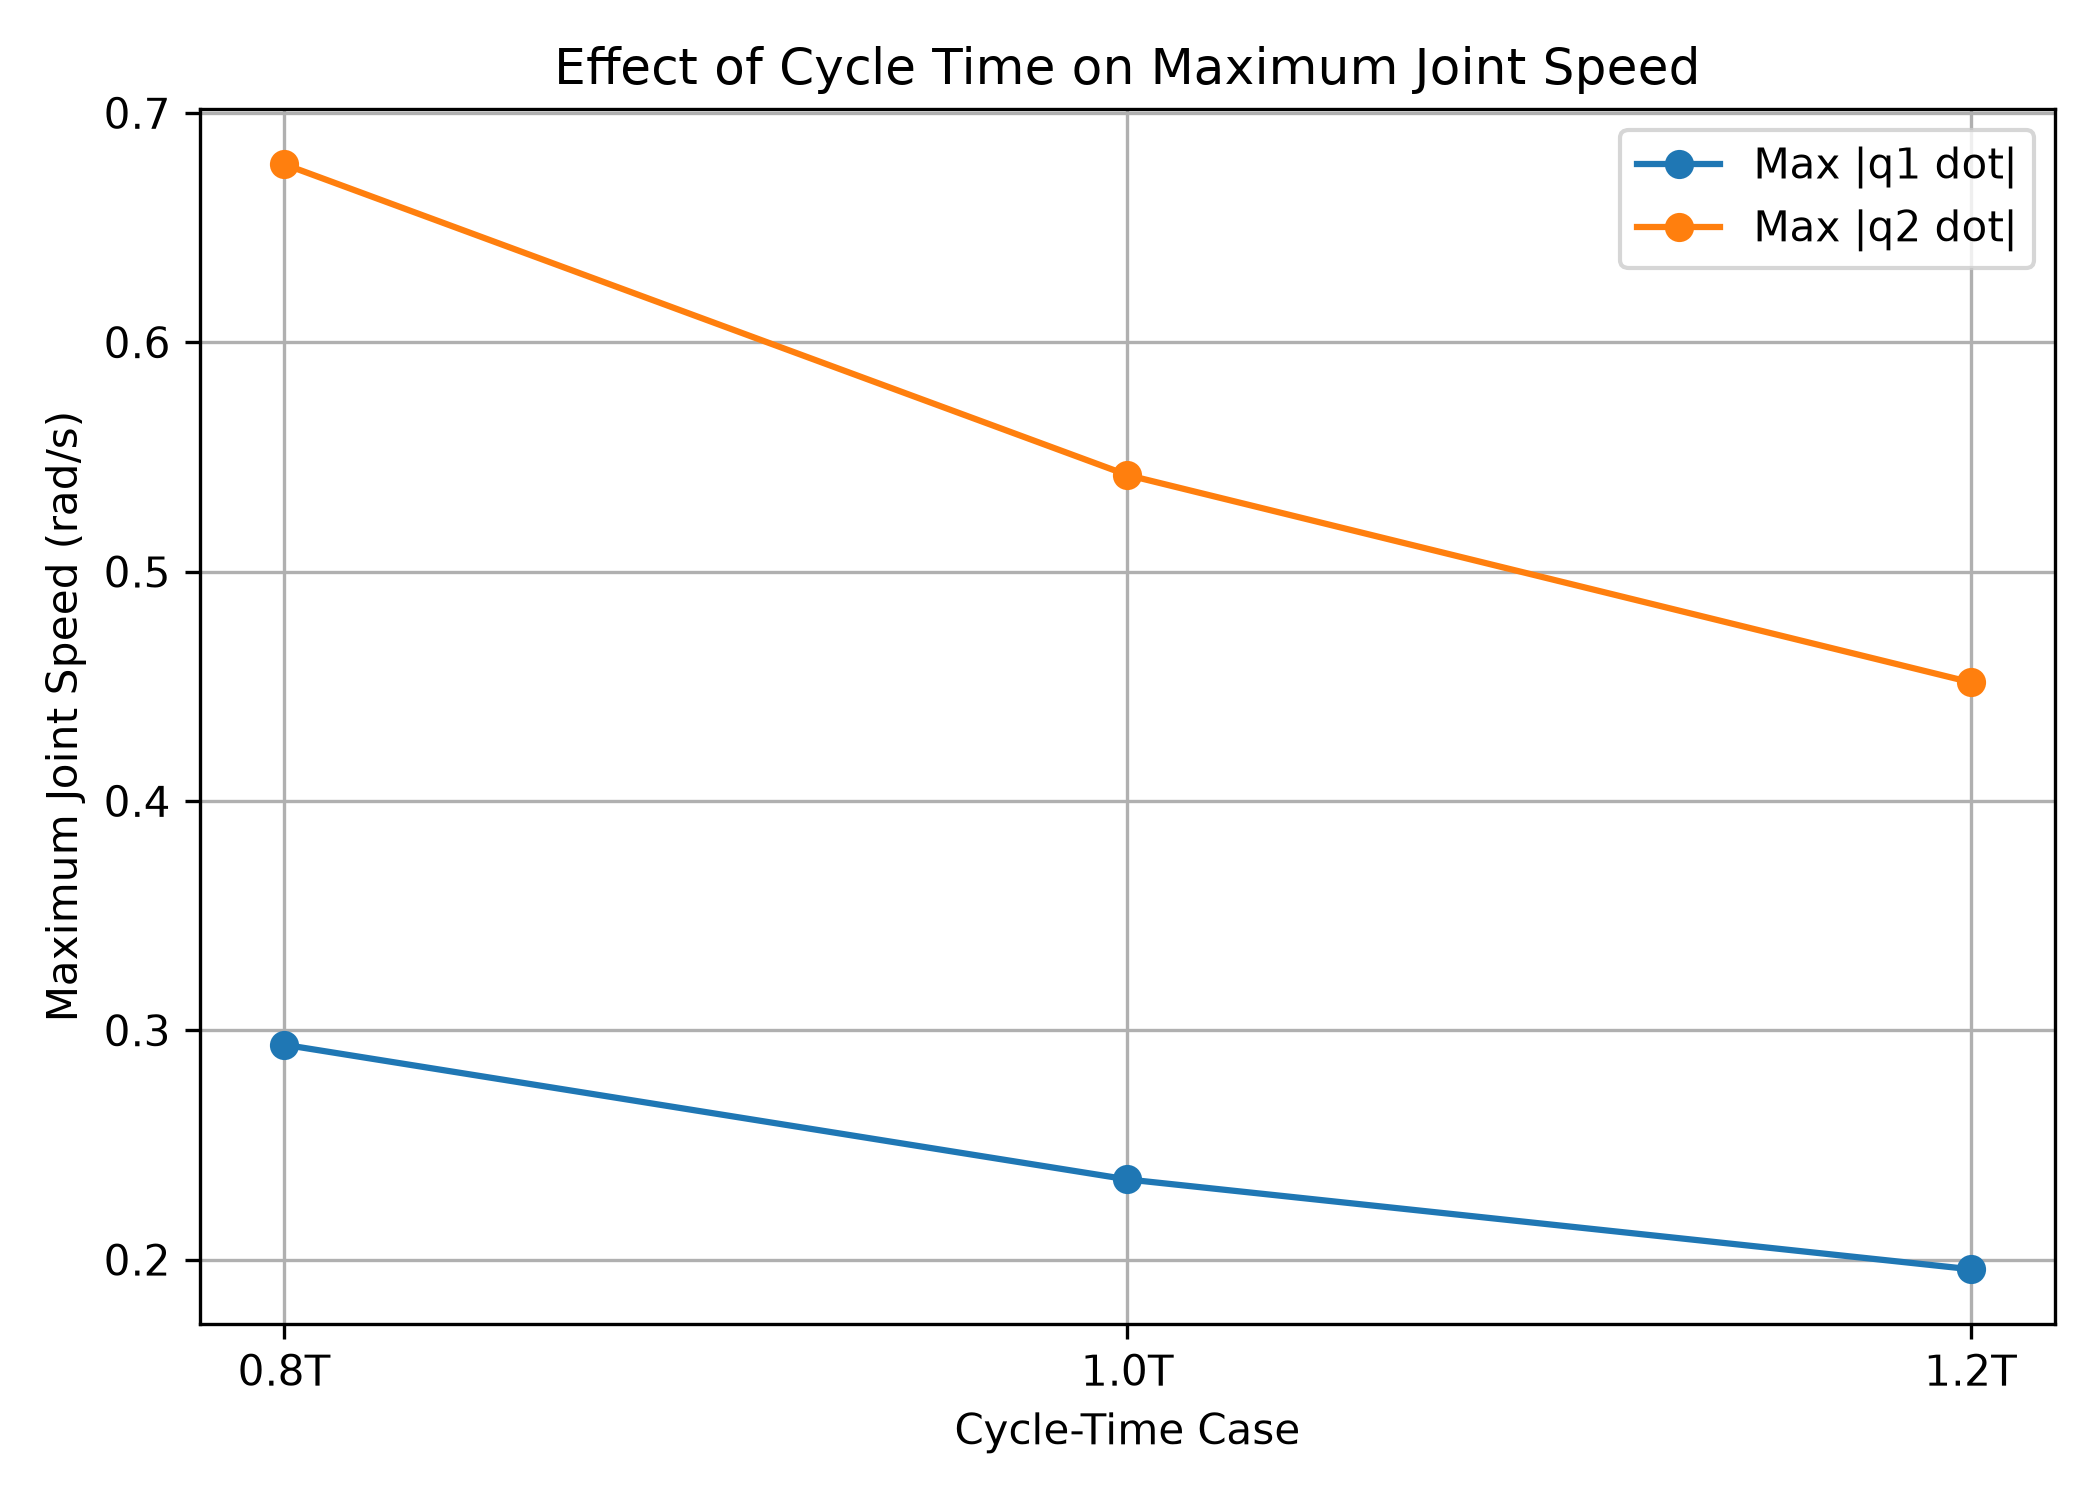
\includegraphics[width=0.60\textwidth]{../results/figures/cycle_time_speed_comparison.png}
\caption{Effect of cycle time on maximum joint angular speed.}
\label{fig:comparison}
\end{figure}

\textbf{Reproducibility and responsible use:}
The submitted Python files reproduce all tabulated values and figures from the assigned \(S=18\) case. The principal assumptions are rigid planar links, ideal joint motion, and the supplied cubic trajectory law; dynamics, actuator torque limits, flexibility, and external disturbances are outside the scope of this kinematic model. Generative AI was used for explanation, coding guidance, debugging support, and report drafting; the equations, program execution, numerical outputs, and verification checks were reviewed and remain the student's responsibility.

% ============================================================
% REFERENCES
% ============================================================
\section*{References}

\begin{enumerate}[label={[\arabic*]},leftmargin=1.1cm,itemsep=3pt]
\item A. Abdennour, ``MATLAB and Python Tools for Engineering Simulation,'' MMM 5162 Modelling and Simulation, Islamic University of Madinah, Topic 1 lecture notes, 2026.

\item A. Abdennour, ``Mini Project 1: Computational Simulation and Parameter Study,'' MMM 5162 Modelling and Simulation, Islamic University of Madinah, Fall Semester 2026.
\end{enumerate}

% ============================================================
% APPENDIX - CODE (not counted in the technical-summary limit)
% ============================================================
\clearpage
\appendix
\section{Python Code}

The executable files submitted with this report are \texttt{robot\_model.py} and \texttt{main\_simulation.py}. The complete source code should be attached as separate executable files in addition to this appendix.

\subsection{robot\_model.py}

\begin{verbatim}
# Paste the final contents of robot_model.py here before submission.
\end{verbatim}

\subsection{main\_simulation.py}

\begin{verbatim}
# Paste the final contents of main_simulation.py here before submission.
\end{verbatim}

\end{document}
